\documentclass[11pt]{beamer}
\usetheme[progressbar=frametitle]{metropolis}
\setbeamertemplate{frame numbering}[fraction]
\useoutertheme{metropolis}
\useinnertheme{metropolis}
\usefonttheme{metropolis}
\usecolortheme{spruce}
\setbeamercolor{background canvas}{bg=white}

\definecolor{mygreen}{rgb}{.125,.5,.25}
\usecolortheme[named=mygreen]{structure}

\title{Floating-point}
%\subtitle{subtitle here}
\author{Van Duc NGUYEN}
\institute{\textbf{Viettel IC Design}}
\date{}
\begin{document}
\metroset{block=fill}
\begin{frame}
\titlepage
\end{frame}
\begin{frame}[t]{Over View}
\begin{enumerate}
\item Introduction
\item Floating-point Representation
\item IEEE 754 floating-point standard for binary
\item Floating-point Arithmetic
\item Implementation in FPGA
\end{enumerate}
\end{frame}
\begin{frame}[t]{1.Introduction}
Why Floating-point?
\begin{enumerate}
\item Advantages
\begin{itemize}
\item Dynamic range\\
with fixed-point $DR_{fxpt}=r^n-1$.\\
with floating-point $DR_{flpt}=\frac{M_{max}*b^{E_{max}}}{M_{min}*b^{E_{min}}}$
\end{itemize}
\item Disadvantages
\begin{itemize}
\item Precision
\item Roundoff error
\item Complex implementation
\end{itemize}
\end{enumerate}
\end{frame}
\begin{frame}[t]{2.Floating-point Representation}
Form represent a floating-point number:\\
\begin{center}
    \begin{figure}[htp]
    \begin{center}
     \includegraphics[scale=.5]{image/fig21}
    \end{center}
    \label{reffig21}
    \end{figure}
\end{center}
With three fields:
\begin{itemize}
\item Sign bit:S (0 is positive and 1 is negative)
\item Fraction:F (Significand or mantissa)
\item Exponent:E
\end{itemize}
Value of floating-point number:{$(-1)^S*{F}*B^{\pm{E}}$}\\
with B
\footnote{The base B is implicit.(base is 2,10..)}
\end{frame}
\begin{frame}{Normalized and Denormalized representation}
\begin{itemize}
\item Normalized:$\pm{1.mmm...m}*B^{\pm{E}}$\\
\item Denormalized:$\pm{0.mmm...m}*B^{E_{min}}$
\end{itemize}
\begin{center}
    \begin{figure}[htp]
    \begin{center}
     \includegraphics[scale=.5]{image/fig2}
    \end{center}
    %\caption{Cái sẽ hiển thị bên dưới hình}
    \label{reffig2}
    \end{figure}
\end{center}
\end{frame}

\begin{frame}[t]{3.IEEE 754 Standard for Binary Floating-point}
The three basic format have bit lengts of 32,64 and 128 bits:
\begin{center}
    \begin{figure}[htp]
    \begin{center}
     \includegraphics[scale=.5]{image/fig20}
    \end{center}
    %\caption{Binary32 format}
    \label{reffig20}
    \end{figure}
\end{center}

For a normalized floating-point number:
\begin{center}
    \begin{figure}[htp]
    \begin{center}
     \includegraphics[scale=.7]{image/fig24}
    \end{center}
    %\caption{Cái sẽ hiển thị bên dưới hình}
    \label{reffig24}
    \end{figure}
\end{center}
Value of floating-point:$\pm{1.f_1f_2f_3f_4...f_l}*2^{\pm{E}}$\\
\end{frame}
\begin{frame}[t]{IEEE 754 Format Paremeter}
\begin{center}
    \begin{figure}[htp]
    \begin{center}
     \includegraphics[scale=.5]{image/fig4}
    \end{center}
    %\caption{Cái sẽ hiển thị bên dưới hình}
    \label{reffig4}
    \end{figure}
\end{center}
\end{frame}
\begin{frame}[t]{Biased Exponent Representation}
IEEE 754 use biased representation for the exponent:
\begin{itemize}
\item Value of exponet= val(E)=E - Bias(Bias is a constant)
\item Bias is computed base on $bias=2^{k-1}-1$ (with k is lengths of bit)
\item For signle precision,k=8 and bias=127,value of E(biased)=val(E)+127.
\end{itemize}
\end{frame}
\begin{frame}[t]{Special value}
IEEE 754 define some special value as NaN,Infinity to represent for underflow,overflow and not a number...\begin{center}
    \begin{figure}[htp]
    \begin{center}
     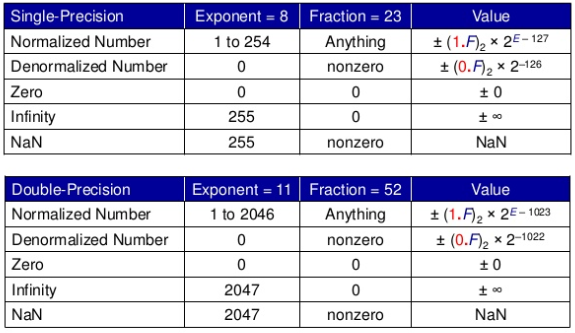
\includegraphics[scale=.5]{image/fig25}
    \end{center}
   %\caption{Cái sẽ hiển thị bên dưới hình}
    \label{reffig25}
    \end{figure}
\end{center}
\end{frame}
\begin{frame}[t]{Rounding Mode}
IEEE 754 standard specifies four rounding modes
\begin{enumerate}
\item Round to nearest even
\item Round toward plus infinity:result is rounded up
\item Round toward minus infinity:result is rounded down
\item Round toward zero:always truncate result
\end{enumerate}
\end{frame}
\begin{frame}[t]{Round to Nearest Even(default rouding mode) }
Normalized result has the form:$\textbf{1.}f_1f_2f_3...f_l\textbf{RS}$
\begin{itemize}
\item $f_l$:last fration bit.
\item round bit\textbf{R}:appears after the last fraction bit $f_l$
\item sticky bit \textbf{S}:is the OR of all remaining addtional bits.
\end{itemize}
Four cases for \textbf{RS}:
\begin{itemize}
\item \textbf{RS=00}:Result is exact,no need for rounding.
\item \textbf{RS=01}:Truncate result by discarding \textbf{RS}
\item \textbf{RS=11}:Increment result by add \textbf{1} to last fraction bit
\item \textbf{RS=10}:Increment or Truncate depend on \textbf{$f_l$}\\
      \begin{itemize}
      \item \textbf{$f_l=0$}:truncate result
      \item \textbf{$f_l=1$}:increment result
      \end{itemize}
\end{itemize}
\end{frame}
\begin{frame}[t]{3.Floating-point Arithmetic}
Basic opreations for floating-point arithmetic:
\begin{center}
    \begin{figure}[htp]
    \begin{center}
     \includegraphics[scale=.4]{image/fig26}
    \end{center}
    %\caption{Cái sẽ hiển thị bên dưới hình}
    \label{reffig26}
    \end{figure}
\end{center}
\end{frame}
\begin{frame}[t]{Addition and Subtration(1):Pseudocode}
    \begin{figure}[htp]
    \begin{center}
     \includegraphics[scale=.37]{image/pesucodeadd}
    \end{center}
    %\caption{Cái sẽ hiển thị bên dưới hình}
    \label{refpesucodeadd}
    \end{figure}
\end{frame}

\begin{frame}[t]{Addition and Subtraction(2):Table of result}
\begin{itemize}
\item Input:X($S_X,E_X,F_X$)và Y($S_Y,E_Y,F_Y$)
\item Output:Z($S_Z,E_Z,F_Z$)
\end{itemize}
\begin{center}
    \begin{figure}[htp]
    \begin{center}
     \includegraphics[scale=.4]{image/fig7}
    \end{center}
    %\caption{Cái sẽ hiển thị bên dưới hình}
    \label{reffig7}
    \end{figure}
\end{center}
\end{frame}
\begin{frame}[t]{Addition and Subtraction(3):Adder Block Diagram}
\begin{center}
    \begin{figure}[htp]
    \begin{center}
     \includegraphics[scale=.5]{image/fig6}
    \end{center}
    %\caption{Cái sẽ hiển thị bên dưới hình}
    \label{reffig6}
    \end{figure}
\end{center}
\end{frame}
\begin{frame}[t]{Multiplication(1):Pseudocode}
\begin{center}
    \begin{figure}[htp]
    \begin{center}
     \includegraphics[scale=.36]{image/pesucodemul}
    \end{center}
    %\caption{Cái sẽ hiển thị bên dưới hình}
    \label{refpesucodemul}
    \end{figure}
\end{center}
\end{frame}
\begin{frame}[t]{Multiplication(2):Multiply Block Diagram}
\begin{center}
    \begin{figure}[htp]
    \begin{center}
     \includegraphics[scale=.3]{image/fig9}
    \end{center}
    %\caption{Cái sẽ hiển thị bên dưới hình}
    \label{reffig9}
    \end{figure}
\end{center}
\end{frame}
\begin{frame}[t]{4.Implementation in FPGA}
The basic operations for floating-point arithmetic performed on FPGA are of type binary32 bit format and it is implemented on the FPGA VCU118-Virtex kit
\begin{center}
    \begin{figure}[htp]
    \begin{center}
     \includegraphics[scale=.5]{image/fig1}
    \end{center}
    %\caption{Cái sẽ hiển thị bên dưới hình}
    \label{reffig1}
    \end{figure}
\end{center}
\begin{center}
    \begin{figure}[htp]
    \begin{center}
     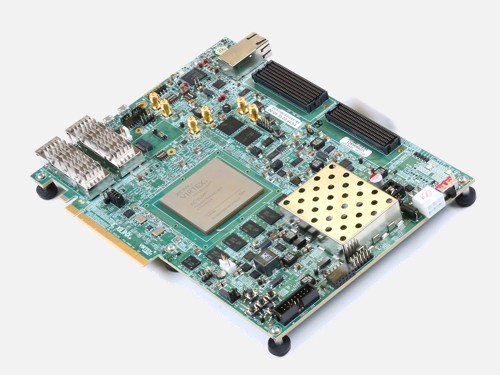
\includegraphics[scale=.3]{image/fig31}
    \end{center}
    %\caption{Cái sẽ hiển thị bên dưới hình}
    \label{reffig31}
    \end{figure}
\end{center}

\end{frame}
\begin{frame}[t]{Implement Addition(1):Unpackage process}
\begin{center}
    \begin{figure}[htp]
    \begin{center}
     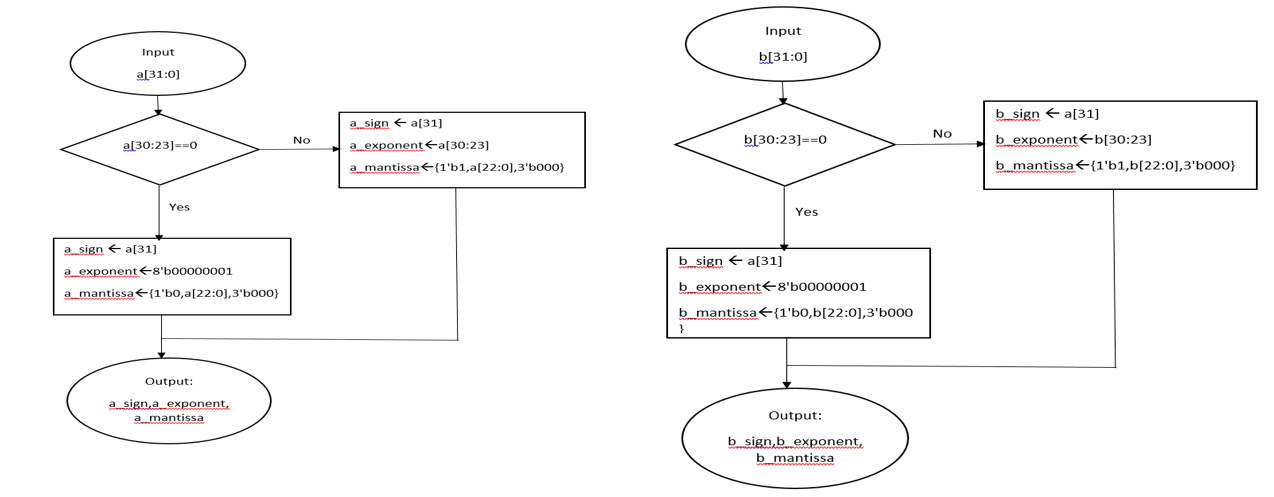
\includegraphics[scale=.33]{image/fig11}
    \end{center}
    %\caption{Cái sẽ hiển thị bên dưới hình}
    \label{reffig11}
    \end{figure}
\end{center}
\end{frame}
\begin{frame}[t]{Implement Addition(2):Block and Flow-chart FSMD}
\begin{center}
    \begin{figure}[htp]
    \begin{center}
     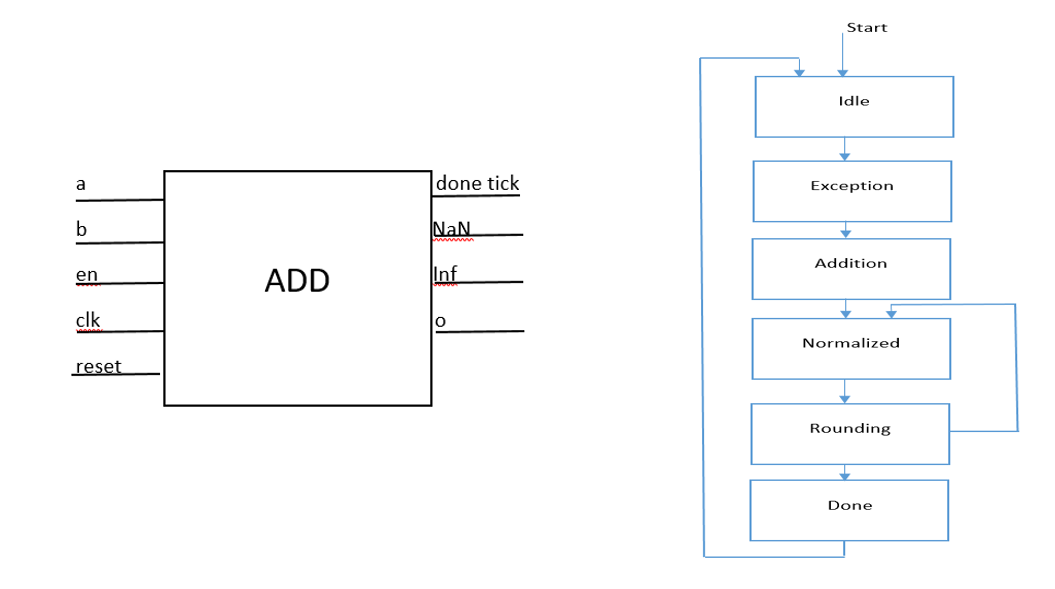
\includegraphics[scale=.35]{image/fig12}
    \end{center}
    %\caption{Cái sẽ hiển thị bên dưới hình}
    \label{reffig12}
    \end{figure}
\end{center}

\end{frame}
\begin{frame}[t]{Implement Addition(3):ASMD diagram}
\begin{center}
    \begin{figure}[htp]
    \begin{center}
     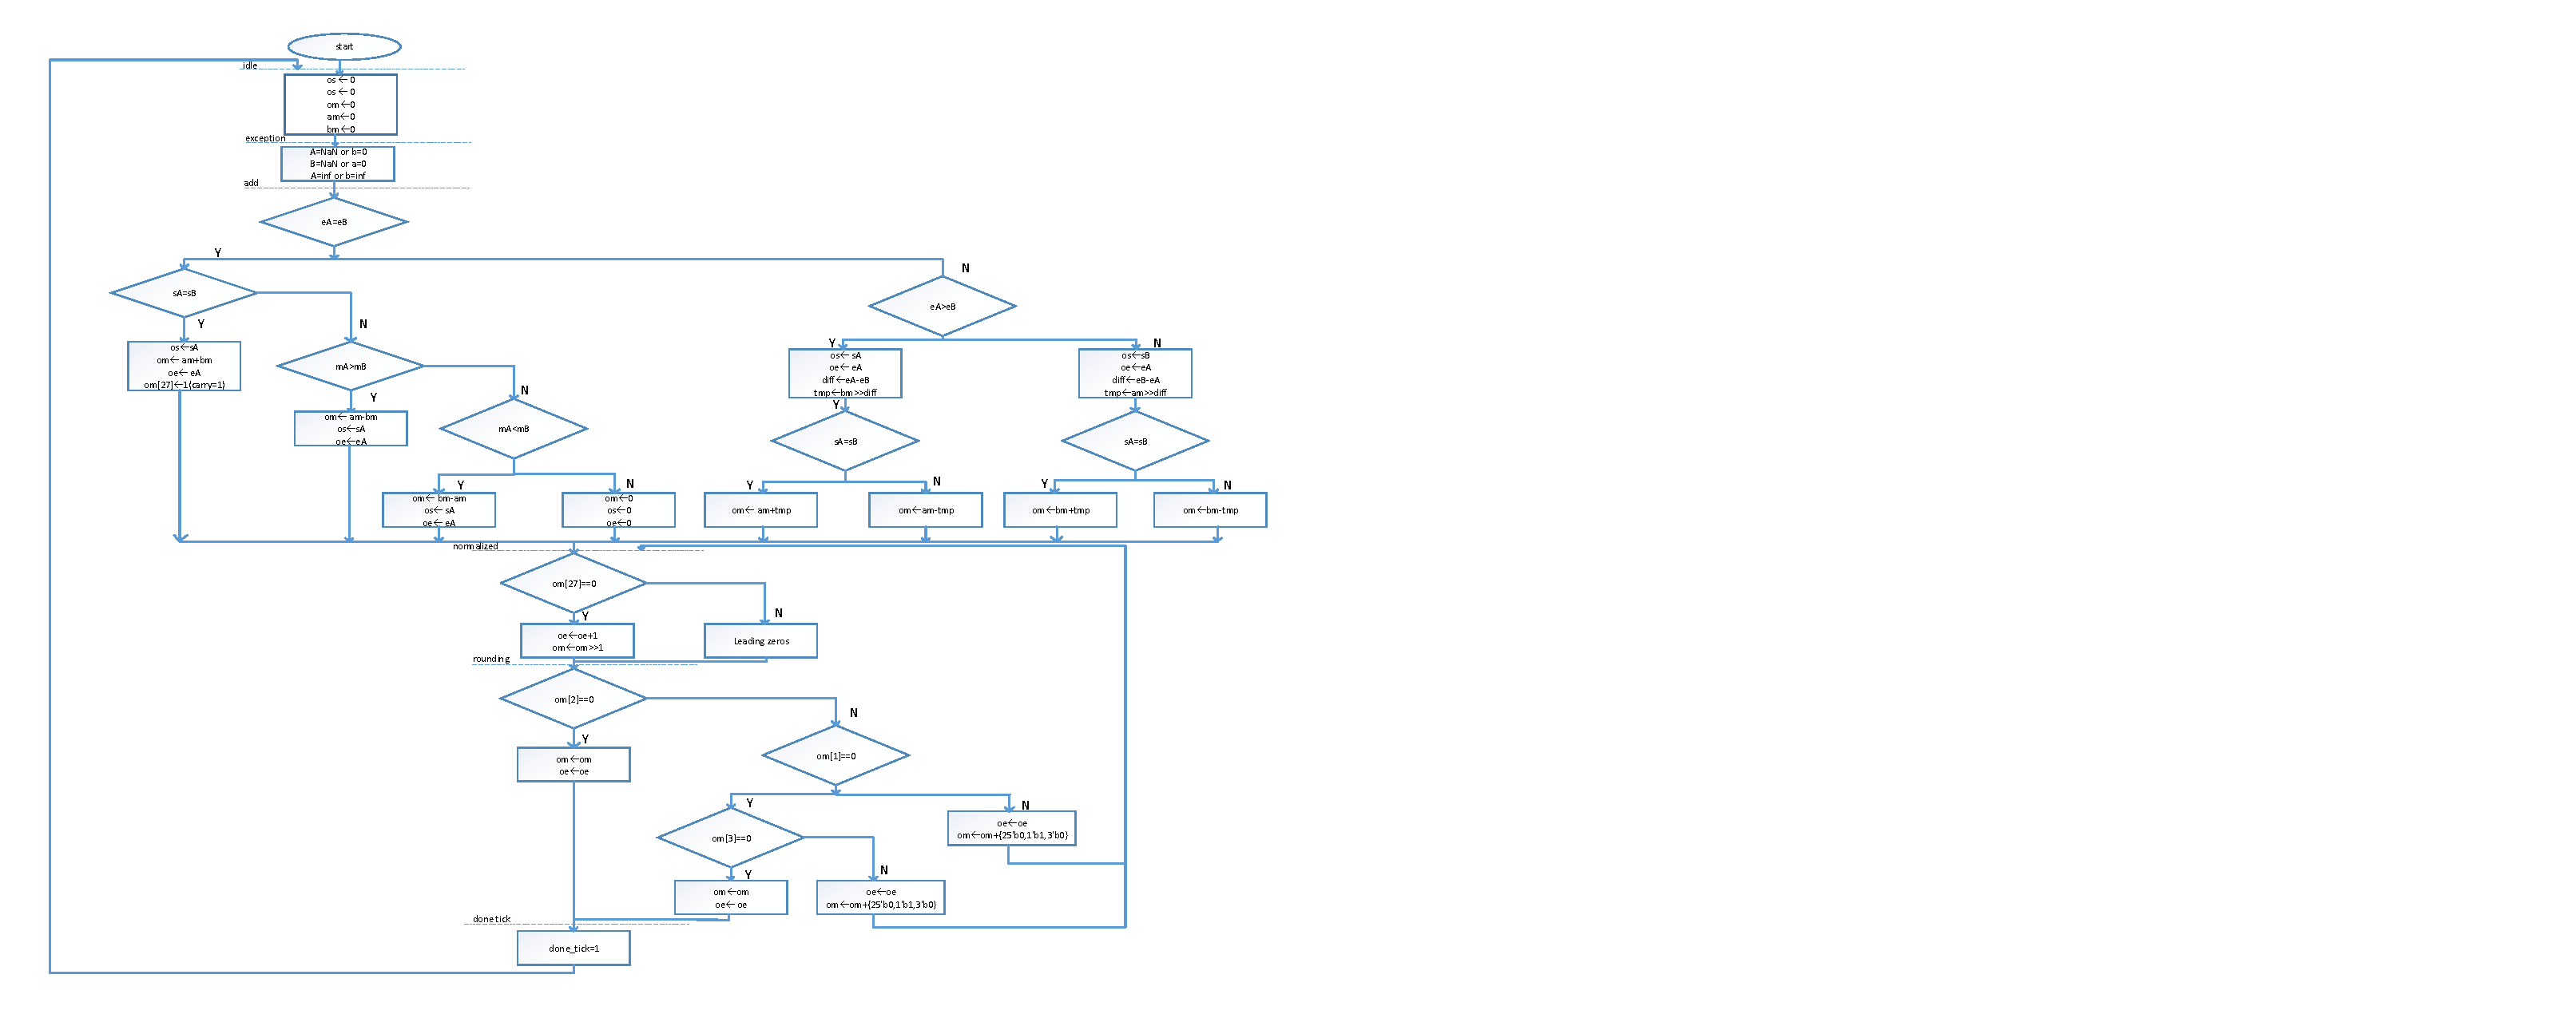
\includegraphics[scale=.33]{image/asmdadd}
    \end{center}
    %\caption{Cái sẽ hiển thị bên dưới hình}
    \label{refasmdadd}
    \end{figure}
\end{center}
\end{frame}
\begin{frame}[t]{Implement Addition(4):Simulation result}
\begin{center}
    \begin{figure}[htp]
    \begin{center}
     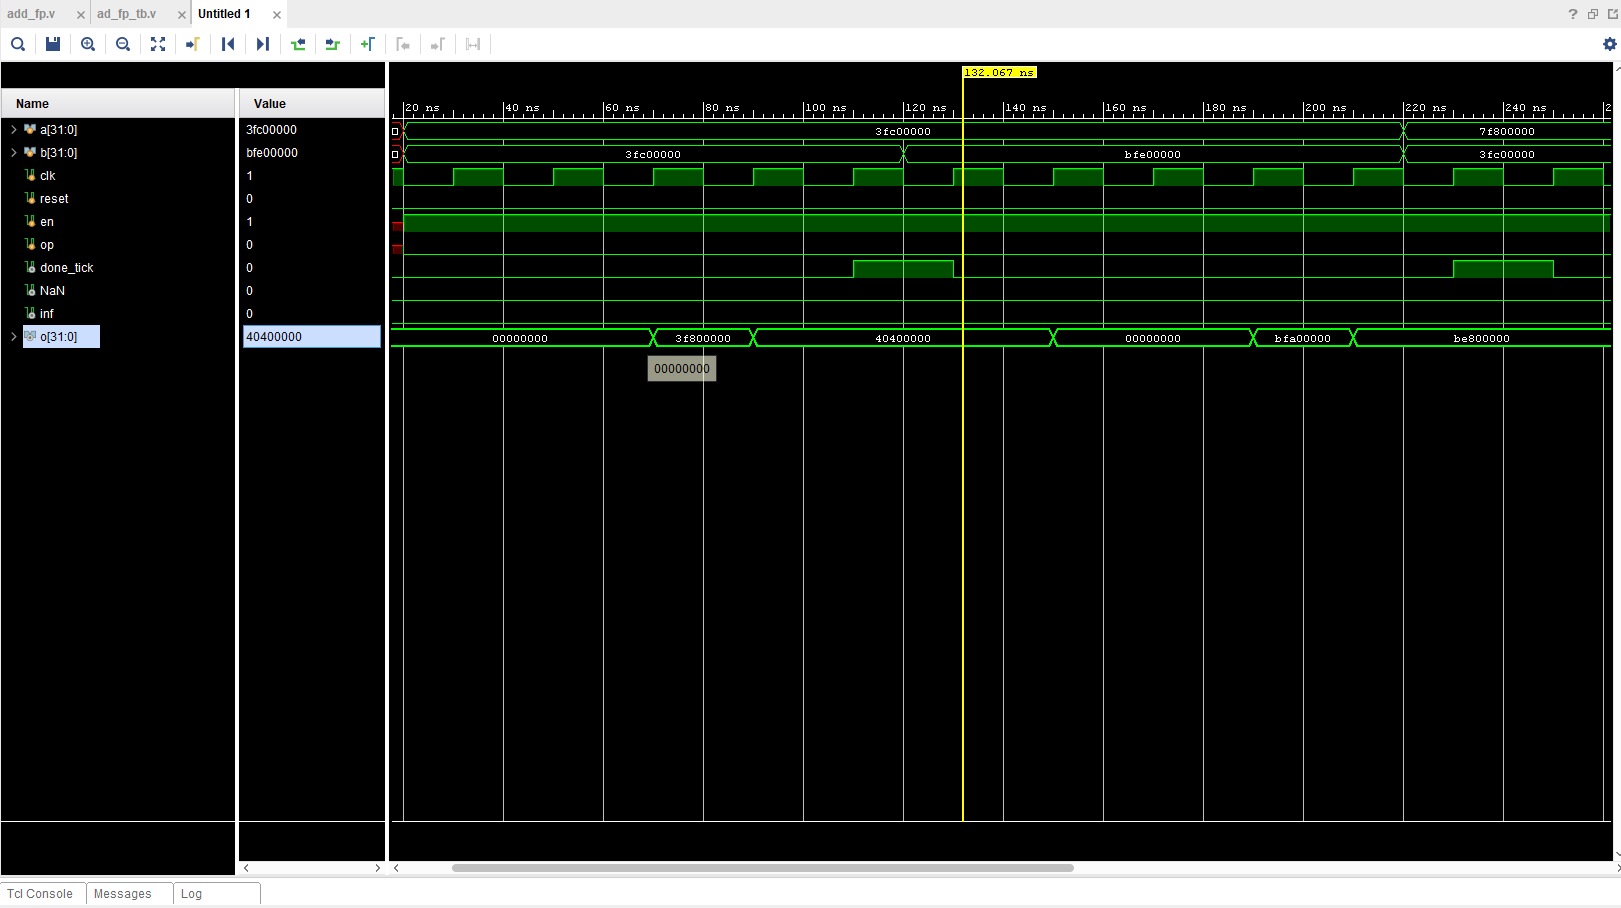
\includegraphics[scale=.26]{image/fig17}
    \end{center}
    %\caption{Cái sẽ hiển thị bên dưới hình}
    \label{reffig17}
    \end{figure}
\end{center}
\end{frame}
\begin{frame}[t]{Implement Addition(5):Timing analysis}
With Frequency clock:100MHz,period=10ns\\
Critical Path :5.217ns(required time-arrival time)
\begin{center}
    \begin{figure}[htp]
    \begin{center}
     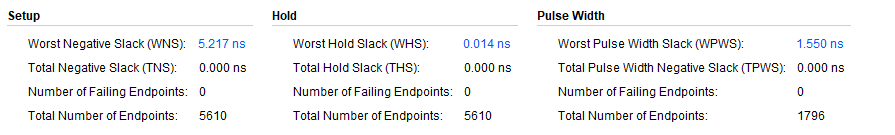
\includegraphics[scale=.5]{image/fig13}
    \end{center}
    %\caption{Cái sẽ hiển thị bên dưới hình}
    \label{reffig13}
    \end{figure}
\end{center}
\end{frame}

\begin{frame}[t]{Implement Multiplication(1):Unpackage process}
\begin{center}
    \begin{figure}[htp]
    \begin{center}
     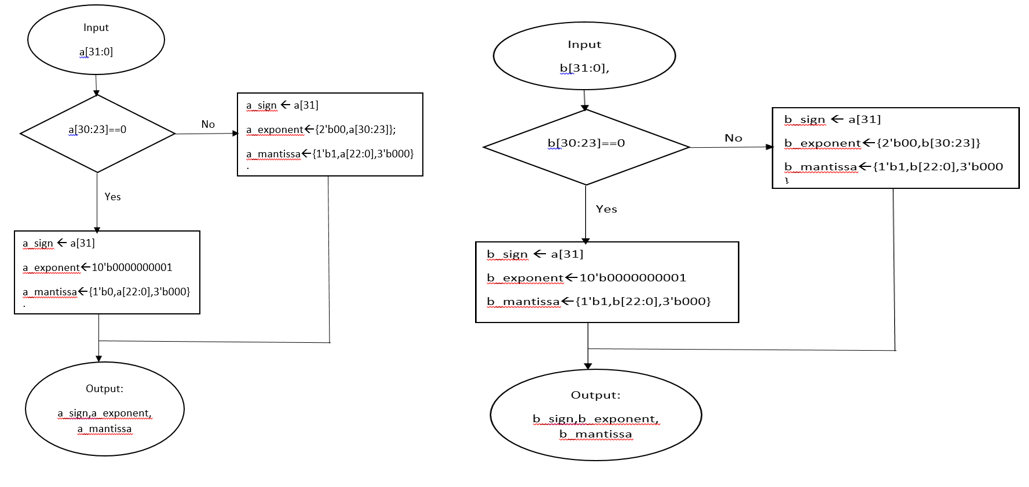
\includegraphics[scale=.37]{image/fig15}
    \end{center}
    \label{reffig15}
    \end{figure}
\end{center}
\end{frame}
\begin{frame}[t]{Implement Multiplication(2):Block and flow-chart FSMD}
\begin{center}
    \begin{figure}[htp]
    \begin{center}
     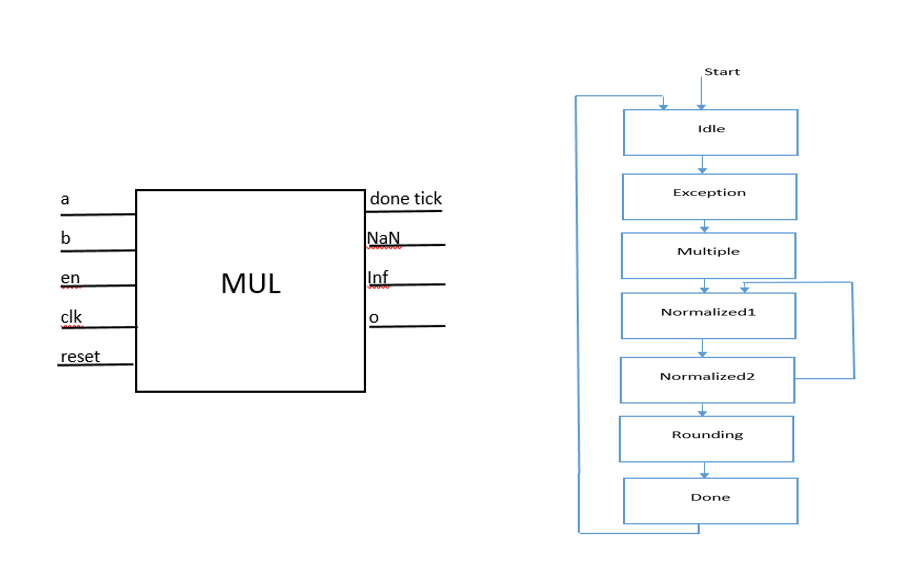
\includegraphics[scale=.4]{image/fig14}
    \end{center}
    \label{reffig14}
    \end{figure}
\end{center}
\end{frame}
\begin{frame}[t]{Implement Multiplication(3):ASMD diagram}
\begin{center}
    \begin{figure}[htp]
    \begin{center}
     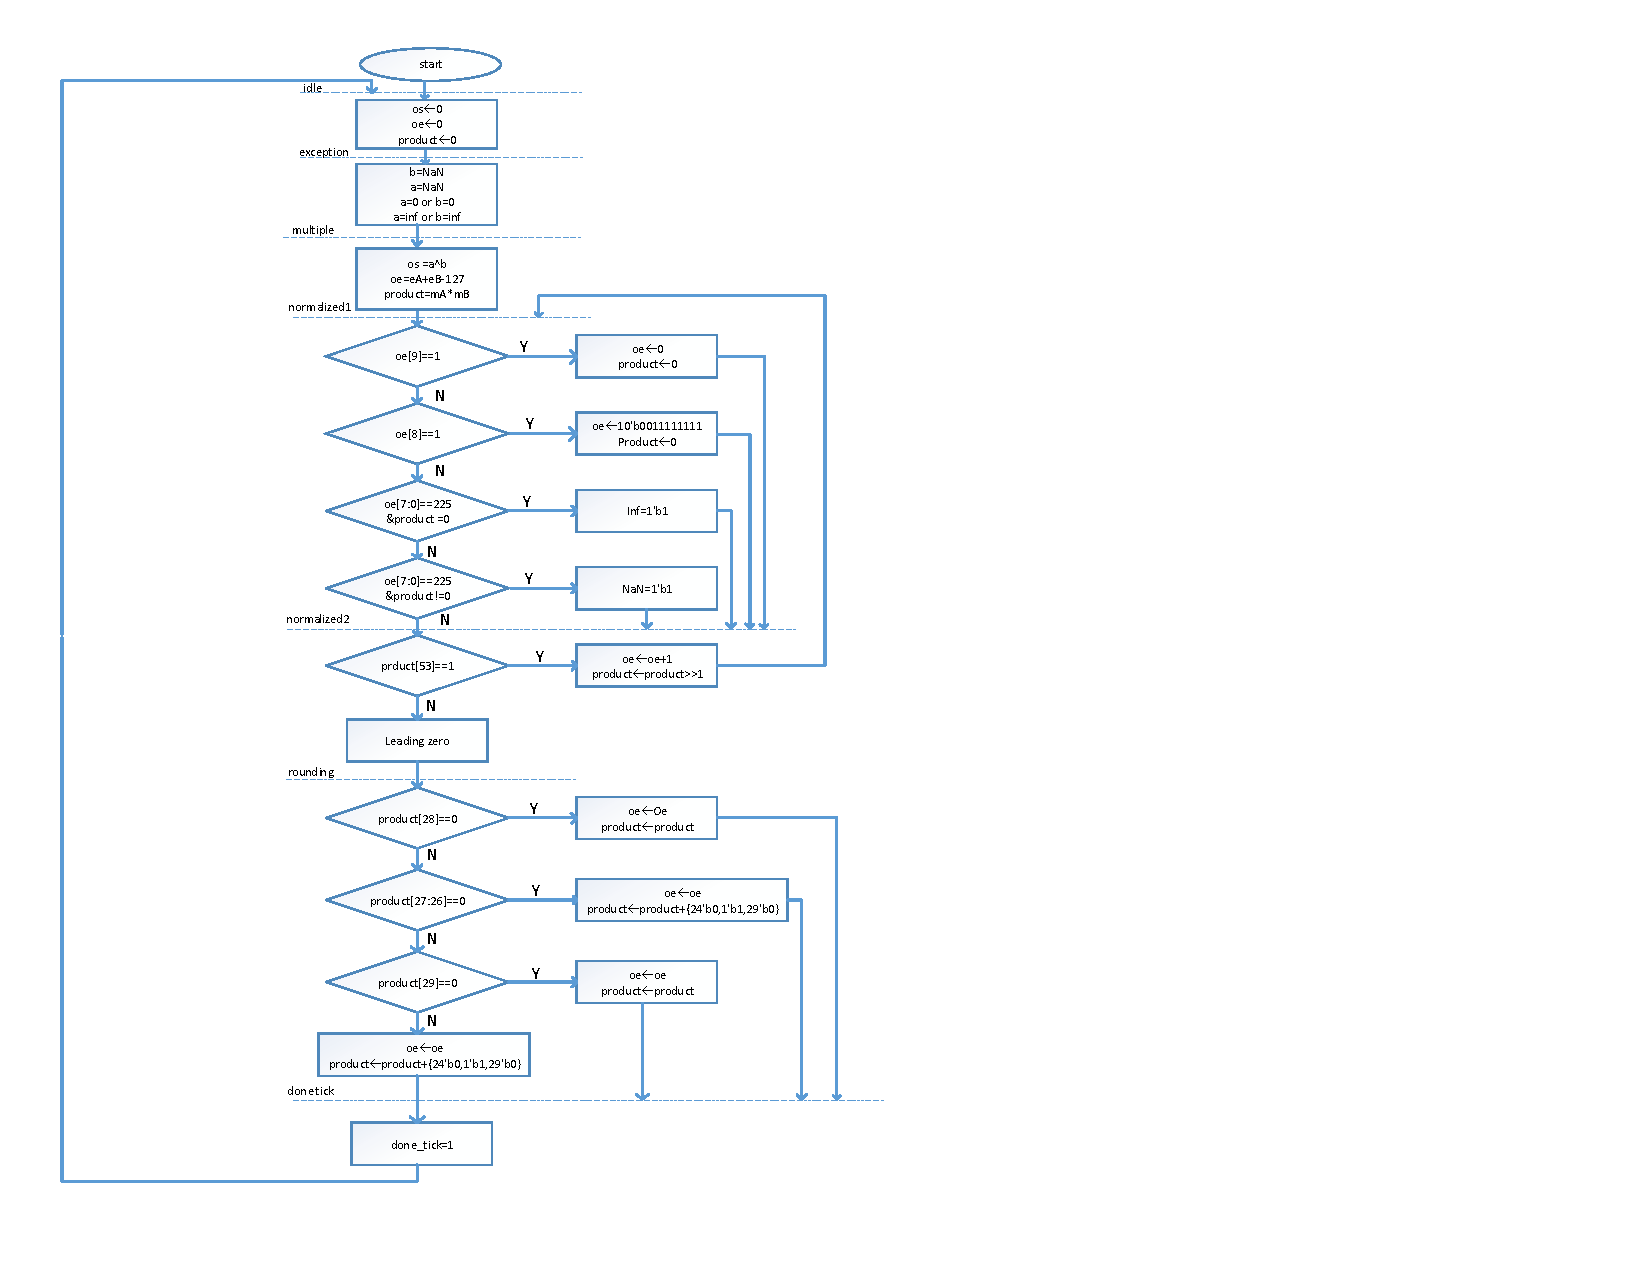
\includegraphics[scale=.37]{image/asmdmul}
    \end{center}
    \label{refasmdmul}
    \end{figure}
\end{center}
\end{frame}
\begin{frame}[t]{Implement Multiplication(4):Simulation result}
\begin{center}
    \begin{figure}[htp]
    \begin{center}
     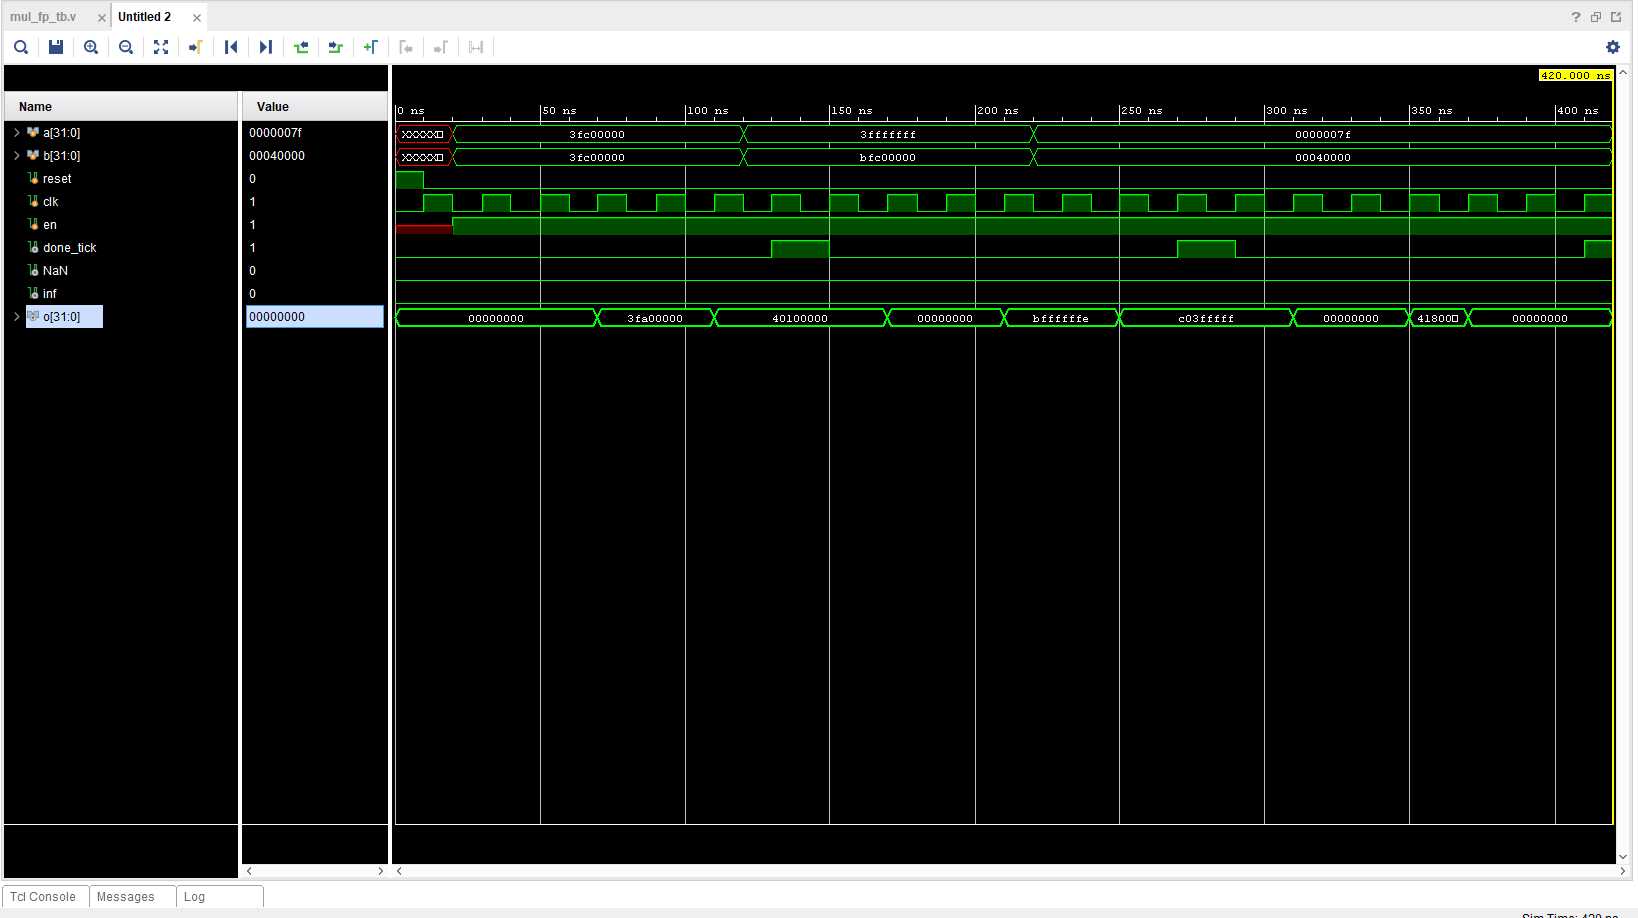
\includegraphics[scale=.25]{image/fig18}
    \end{center}
    \label{reffig18}
    \end{figure}
\end{center}
\end{frame}
\begin{frame}[t]{Implement Multiplication(5):Timing analysis}
With Frequency clock:100MHz,period=10ns\\
Critical Path :5.029ns(required time-arrival time)
\begin{center}
    \begin{figure}[htp]
    \begin{center}
     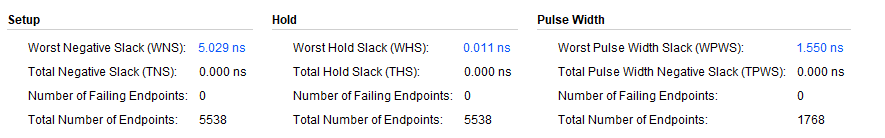
\includegraphics[scale=.37]{image/fig16}
    \end{center}
    \label{reffig16}
    \end{figure}
\end{center}
\end{frame}
\begin{frame}{Conclusion}

\end{frame}
\end{document}
